
%
% template for Bachelor thesis
% LIACS
% January 7, 2019
%

\documentclass[12pt]{article}

% include some packages
\usepackage[left=2cm,right=2cm,top=2cm,bottom=3cm]{geometry}
\usepackage{graphicx}
\usepackage{tikz}
\usepackage{tikz-cd}
\usetikzlibrary{shapes,backgrounds,calc,arrows}
\usepackage{microtype}
\usepackage{amsmath}
\usepackage[utf8]{inputenc}
\usepackage{amsfonts}
\usepackage{amssymb}
\usepackage{amsthm}

\newtheorem{definition}{Definition}

\usepackage{bbm}
\usepackage{geometry}
\usepackage{csquotes}
\usepackage[hidelinks]{hyperref}
\usepackage{mathtools}
\usepackage{parskip}

\usepackage{mathtools}
\newcommand{\defeq}{\vcentcolon=}
\newcommand{\eqdef}{=\vcentcolon}

\DeclareMathOperator{\Ima}{Im}
\DeclareMathOperator{\sech}{sech}
\renewcommand{\P}{\mathcal{P}}
\newcommand{\R}{\mathbb{R}}
\newcommand{\C}{\mathbb{C}}
\newcommand{\N}{\mathbb{N}}
\newcommand{\E}[1]{\mathbb{E}\{#1\}}
\newcommand{\Q}{\mathbb Q}
\newcommand{\Z}{\mathbb{Z}}
\newcommand{\1}{\mathbbm{1}}
\newcommand{\ua}{\nearrow}
\newcommand{\da}{\searrow}
\newcommand{\eps}{\varepsilon}
\newcommand{\dx}{\mathrm{d}x}
\newcommand{\B}{\mathcal{B}}
\newcommand{\F}{\mathcal{F}}
\newcommand{\T}{\mathbb{T}}
\newcommand{\V}{\mathcal{V}}
\newcommand{\U}{\mathcal{U}}
\newcommand{\id}{\text{id}}
\newcommand{\I}{\mathcal{I}}
\newcommand{\A}{\mathcal{A}}
\newcommand{\J}{\mathcal{J}}
\newcommand{\G}{\mathcal{G}}
\renewcommand{\L}{\mathcal{L}}
\newcommand{\specepsilon}{\mathcal{E}}
\newcommand{\M}{\mathcal{M}}
\newcommand{\II}{\textbf{II}}
\newcommand{\bigo}{\mathcal{O}}
\usepackage[setpagesize=false,colorlinks=true,linkcolor=blue,urlcolor=red,pdftitle={An Interesting Title for a Thesis},pdfauthor={Your Name}]{hyperref}
\setlength\parindent{0pt}

\begin{document}
\thispagestyle{empty}


\includegraphics{logoleiden}

\vspace{-2.5cm}\hfill \begin{huge}\textbf{Opleiding Informatica}\end{huge}

\vspace{5cm}
\begin{Large}
\hfill Simplicial Coalgebras

\vspace*{3mm}

\hfill for Concurrent Regular Languages

\vspace*{14mm}

\hfill Hessel Sieburgh
\end{Large}

\vspace*{6.0cm}

\begin{large}

Supervisors:\\
Henning Basold \& 
Marton Hablicsek


\vspace*{2.8cm}
BACHELOR THESIS

\vspace*{5mm}
Leiden Institute of Advanced Computer Science (LIACS)\\
\href{www.liacs.leidenuniv.nl}{\underline{\texttt{www.liacs.leidenuniv.nl}}}\hfill 01/07/2025
\end{large}

\newpage



% abstract and references should fit on one page
\begin{abstract}
\noindent
This is where you write an abstract that concisely summarizes your thesis.
Keep it short. No references here --- exceptions do occur.
\end{abstract}

\bigskip

\thispagestyle{empty}
\tableofcontents
\thispagestyle{empty}
%Some (very few) people like a list of tables:
%\listoftables
%And some (even fewer) like a list of figures:
%\listoffigures

\clearpage
\setcounter{page}{1}

\section{Introduction} \label{introduction}

In this section we give an introduction to the problem addressed in this thesis.


\subsection{The situation}

Sections may include subsections.

To make sure that this document renders correctly, execute these commands:
\begin{quote}
\begin{verbatim}
pdflatex thesis
bibtex thesis
pdflatex thesis
pdflatex thesis
\end{verbatim}
\end{quote}
Here, the \verb|pdflatex| command may need to be executed three times in order to generate the table of contents and so on. 
Note that a good thesis has figures and tables; examples can be found in Figure~\ref{afigure} and Table~\ref{atable}. And every thesis has references, like~\cite{whatagreatpaper}.

\begin{figure}[!htbp]
\begin{center}
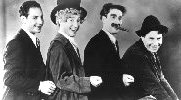
\includegraphics[height=2cm]{marxbrothers2}
\end{center}
\caption{Every thesis should have figures. Source: \href{www.marxbrothers.org}{\underline{\texttt{www.marxbrothers.org}}}.}\label{afigure}
\end{figure}

\begin{table}[!htbp]
\begin{center}
\begin{tabular}{l|l}
Column A & Column B\\
\hline
Point 1 & Good\\
Point 2 & Bad
\end{tabular}
\end{center}
\caption{Every thesis should have tables.}\label{atable}
\end{table}

Final reminder: this template is just an example, if you want you can make adjustments; also discuss with your supervisor which layout he or she likes. But the front page should be as it is now.

TODO: quite a lot!

\subsection{Thesis overview}
It is recommended to end the introduction with an overview of the thesis. This chapter contains the introduction; Section~\ref{definitions} includes the definitions; Section~\ref{relatedwork} discusses related work; Section~\ref{experiments} describes the experiments and their outcome; Section~\ref{conclusions} concludes. By the way, different section titles are certainly possible.

Also, produce a nice sentence with ``bachelor thesis'', LIACS and the names of the supervisors.
\section{Notes}
\begin{definition}{Ranked term graph}

A \emph{ranked term graph} consists of:
\begin{itemize}
\item A directed acyclic graph (DAG) $g$,
\item A \emph{rank} $(d_r, d_v) \in \N^2$. Denoting the size of the root and target interfaces,
\item Let $[n] \defeq \{1,2,\dots, n\}$. Maps $r: [d_r] \to \P(g)$ and $v: [d_v] \to \P(g)$, where $r([d_r])$ consists of minimal vertices of $g$ and $v([d_v])$ consists of maximal vertices called the \emph{root} and \emph{variable} maps.
\end{itemize}
\end{definition}

\subsection{Monoidal Structure}
\begin{definition}
Let $G = (g^G, (d_r^G, d_v^G), r^G, v^G)$, $F = (g^F, (d_r^F, d_v^F), r^F, v^F)$ be ranked term graphs. We define a monoidal product functor as:
$$G \oplus F = \left(g^G \sqcup g^F, (d_r^G + d_r^F, d_v^G + d_v^F), r', v'\right)$$
Where $r'$, $v'$ are the concatenations of $r^G$ and $r^F$, $v^G$ and $v^F$ respectively:
\begin{align*}
    r'(k) = \begin{cases} 
      r^G(k) & k\leq d^G_r\\
      r^F(k-d^G_r)& d^G_r < k \leq d^G_r + d^F_r \\
   \end{cases}
\end{align*}

\begin{align*}
    v'(k) = \begin{cases} 
      v^G(k) & k\leq d^G_v\\
      v^F(k-d^G_v)& d^G_v < k \leq d^G_v + d^F_v \\
   \end{cases}
\end{align*}
\end{definition}

\subsection{Composition of Morphisms}
\begin{definition}
Let $G = (g^G, (d_r^G, d_v^G), r^G, v^G)$, $F = (g^F, (d_r^F, d_v^F), r^F, v^F)$ be ranked term graphs such that $d_v^G = d_r^F$, their composition is defined as follows:
$$G\circ F = (H, (d_r^G, d_v^F), r^G, v^F)$$
Where $H = g^G\sqcup g^F \sqcup\{(x,x') \in g^G\times g^F | \exists i\in[d_v^G]. x\in v^G(i) \wedge x'\in r^F(i)\}$ which is equal to the two union of the two graphs with added arrows going from roots to variables which are equally numbered.
\end{definition}

A category with ranked term graphs as morphisms, $\N$ as the set of objects, the disjoint union as monoidal product, and the defined composition of morphisms gives a monoidal category.
\newpage

\subsection{Simplicial set}
To get a simplicial set we need an extra piece of equipment: parallel composition with identification of the interfaces.
\begin{definition}
    Let $G$, $F$ be ranked term graphs of equal rank $(d_r, d_v)$. Then:
    $$G\otimes F = (g^G\sqcup g^F, (d_r, d_v), r^G \sqcup r^F, v^G \sqcup v^F)$$
\end{definition}

And lastly we are able to identify two consecutive interface points:

\begin{definition}
    Let $G$ be a ranked term graph of rank $(n,n)$, define $p_m$ to be the identification of the $m, m+1$-th interface points, for $m\in\{0\}\cup[n]$
    \begin{align*}
        p_m(G) = (g, (n-1, n-1), r', v')
    \end{align*}
    Where we have:
    \[
    r'(k) = \begin{cases}
        r(k) & k < m\\
        r(m) \cup r(m+1) & k = m\\
        r(k + 1) & m < k < n
    \end{cases}
    \]
        \[
    v'(k) = \begin{cases}
        v(k) & k < m\\
        v(m) \cup v(m+1) & k = m\\
        v(k + 1) & m < k < n
    \end{cases}
    \]
\end{definition}

\newpage
\section{Related Work}\label{relatedwork}

\section{Experiments}\label{experiments}

\section{Conclusions and Further Research}\label{conclusions}

\bibliographystyle{alpha}
\bibliography{bibliography}
\addcontentsline{toc}{section}{References}


%\appendix
%appendices here --- if any

\end{document}
